\documentclass[conference]{IEEEtran}
\IEEEoverridecommandlockouts
\usepackage[utf8]{inputenc}
\usepackage[T1]{fontenc}
\usepackage{amsmath,amssymb}
\usepackage{graphicx}
\usepackage{booktabs}
\usepackage{array}
\usepackage{cite}
\usepackage{url}
\usepackage[hidelinks]{hyperref}
\graphicspath{{../figs/}}
% Shared notation for the IEEE paper, the LNCS paper and the full report.
% Packages are loaded by each main.tex; this file only defines commands.
\providecommand{\QUBO}{QUBO}
\providecommand{\HUBO}{HUBO}
\newcommand{\Lam}{\ensuremath{\Lambda}}
\newcommand{\Lsafe}{\ensuremath{\Lambda_{\mathrm{safe}}}}
\newcommand{\Fset}{\ensuremath{\mathcal{F}}}
\newcommand{\Popt}{\ensuremath{P(\mathrm{opt})}}
\newcommand{\btrue}{\ensuremath{\mathrm{benefit}_{\mathrm{true}}}}
\newcommand{\Tstar}{\ensuremath{T^{\ast}}}
\newcommand{\Wstar}{\ensuremath{W^{\ast}}}
\newcommand{\degC}{\ensuremath{^{\circ}}C}
\newcommand{\gap}{\ensuremath{\Delta(s{=}1)}}
\newcommand{\code}[1]{\texttt{#1}}
\newcommand{\repo}{\texttt{s-siyanwal/q\_uhi}}
\newcommand{\sha}{\texttt{e649582}}
\newcommand{\blob}[1]{\url{https://github.com/s-siyanwal/q_uhi/blob/claude/clever-gates-ezote4/#1}}
% Unicode that appears in method names copied from the CSVs
\DeclareUnicodeCharacter{03B1}{\ensuremath{\alpha}}
\DeclareUnicodeCharacter{039B}{\ensuremath{\Lambda}}
\DeclareUnicodeCharacter{00B7}{\ensuremath{\cdot}}
\DeclareUnicodeCharacter{00D7}{\ensuremath{\times}}
\DeclareUnicodeCharacter{2264}{\ensuremath{\leq}}
\DeclareUnicodeCharacter{2265}{\ensuremath{\geq}}
\DeclareUnicodeCharacter{2212}{\ensuremath{-}}
\DeclareUnicodeCharacter{03BC}{\ensuremath{\mu}}
\DeclareUnicodeCharacter{2013}{--}
\DeclareUnicodeCharacter{2014}{---}
\DeclareUnicodeCharacter{2192}{\ensuremath{\rightarrow}}


\begin{document}
\title{Constraint Encodings, Not Annealers, Dominate QUBO/HUBO Siting for Urban Heat-Island Interventions}
\author{\IEEEauthorblockN{The \code{quhi} project}
\IEEEauthorblockA{Repository \repo{}, commit \sha}}
\maketitle

\begin{abstract}
We site parks, water bodies and cool pavement on synthetic 50\,m city grids. Each instance is a
constrained binary program, encoded as a \QUBO{} or \HUBO{} and scored on exact saturating cooling
physics against a HiGHS-certified optimum. A slack-bit penalty \QUBO{} with a corrected weight has
the MILP optimum as its ground state on all 11 exhaustively enumerated instances. The second-order
Taylor \QUBO{} loses 10.3\% of the achievable cooling at 300\,m reach, where the cubic \HUBO{} loses
at most 0.02\% and a least-squares-fitted \QUBO{} at most 0.42\%. The final annealing gap scales as
$1/\Lam$ with the penalty weight. Constraint-preserving Dicke-XY QAOA reaches a mean $\Popt$ of
0.43 at depth 6, against 1.00 for feasible-space simulated annealing. Path-integral Monte Carlo
restricted to the feasible set passes a pre-committed comparability bar (benefit 0.981), but it
made 3.6$\times$ more proposals than feasible-space annealing; at equal proposals it scores 0.983
against 0.988. HiGHS certifies every hard-family instance in 0.77\,s on average. Encodings and
constraint handling, not the choice of annealer, decide the outcome. We observe no quantum or
quantum-inspired advantage.

\end{abstract}
\begin{IEEEkeywords}
QUBO, HUBO, penalty methods, QAOA, simulated quantum annealing, urban heat island, benchmarking
\end{IEEEkeywords}

%======================================================================
\section{Introduction}\label{sec:intro}
Urban planners who want to cool a city choose a small number of sites for parks, water and
reflective pavement. The choice is a binary program with a budget, a one-option-per-cell rule and,
often, an equity rule that every district receives something. Because such programs can be written
as \QUBO{}s, they are routinely offered as applications for quantum annealers and gate-model QAOA.
Whether that is useful depends on how the constraints and the physics are encoded, and on what the
quantum method is compared with.

We report a negative result with a precise cause. Using an audited open toolkit (\code{quhi}) and
certified optima throughout, we find:
\begin{itemize}
\item the certified slack-penalty \QUBO{} is exact (E1), but its penalty sets the analog gap, which
scales as $1/\Lam$ (E6);
\item Taylor truncation to a \QUBO{} misrepresents long-reach cooling (10.3\% loss at 300\,m), which a
cubic \HUBO{} or a fitted \QUBO{} avoids (E2);
\item constraint-preserving QAOA fixes feasibility but not quality: $\Popt=0.43$ at $p=6$ against 1.00
for feasible-space SA (E8b);
\item feasible-space path-integral Monte Carlo (FeasibleSQA) passes a pre-committed comparability bar,
but at equal proposals it trails feasible-space SA, 0.983 against 0.988 (E12, E12b);
\item HiGHS certifies every hard-family instance in 0.77\,s on average and a $16\times16$
LST-shaped tile in 1.67\,s (E12b, E13).
\end{itemize}
The success criterion, fixed before the quantum experiments, is demanding by design: at matched
wall-clock on certified instances, a method must meet the greedy planner and HiGHS MILP on both a
park family and a mix + equity family. Matching simulated annealing is not enough.

%======================================================================
\section{Problem}\label{sec:problem}
\subsection{Cooling model}
A city is a grid of 50\,m cells~\cite{zhou2023}. Variable $x_v$, $v=(i,o)$, places option $o$
(park, water body, cool pavement) on candidate cell $i$. Option $o$ at cell $i$ cools target cell
$k$ by $e_{ik}=A_o\exp(-d_{ik}/L_o)$; the defaults are 1.5\,\degC{}/100\,m for parks,
2.0\,\degC{}/80\,m for water and 0.6\,\degC{}/30\,m for cool pavement, at 3, 5 and 1 cost units.
Overlapping effects saturate:
\begin{equation}
\Delta T_k=\Delta T_{\max}\Bigl[1-\prod_v(1-p_{kv}x_v)\Bigr],
\label{eq:sat}
\end{equation}
where $p_{kv}=\min(e_{kv},\Delta T_{\max})/\Delta T_{\max}$
and $\Delta T_{\max}=3$\,\degC{}. We minimise the exposure-weighted temperature
$f(x)=\sum_k w_k(T^0_k-\Delta T_k)$ with $w_k=0.7\,\mathrm{pop}_k/\sum\mathrm{pop}+0.3/N$.
Truncating inclusion--exclusion at order $K$ gives an additive model ($K{=}1$), a \QUBO{} ($K{=}2$,
a pessimistic bound by Bonferroni) or a cubic \HUBO{} ($K{=}3$). An optional park-block synergy
adds quartic terms.

\subsection{Constraints and scoring}
Constraints are an integer budget, at most one option per cell and optionally at least one
intervention per district. Without equity, $-f$ is monotone submodular, so greedy enjoys a
$(1-1/e)$ guarantee~\cite{nemhauser1978}. A plan's $\btrue$ is its exact-physics cooling divided by
that of the MILP plan (infeasible $=0$); $\Popt$ is the fraction of runs returning the certified
optimum.

\subsection{Why an audit came first}
The earlier code base shipped energies of order $10^{10}$ and an all-zero SQA plan. The audit traced
these to inequality constraints encoded as equalities in raw m$^2$ (coefficient ratio
$1.72\times10^{9}$ against 2.0), an SQA action with $\beta$ instead of $\beta/P$ (single-qubit
$\langle\sigma_z\rangle=-0.997$ against the exact $-0.545$), and a penalty theorem that is false for
non-integer data; 19 of its 163 tests fail. Table~\ref{tab:audit} lists the findings; none of the
legacy numbers is used as evidence here. The legacy documents also appealed to asymptotic
quantum-annealing results for disordered chains~\cite{santoro2002}; E6 shows why such results do not
transfer to dense, penalty-dominated \QUBO{}s.

\begin{table}[!t]
\centering\caption{Findings of the legacy audit (F1--F7).}\label{tab:audit}
\scriptsize% typed from docs/AUDIT.md
\begin{tabular}{lp{0.36\linewidth}p{0.46\linewidth}}
\toprule
& finding & evidence (docs/AUDIT.md, results/audit/audit.json) \\
\midrule
F1 & inequalities encoded as equalities, in raw m$^2$ & $|Q|_{\max}=1.72\times10^{9}$ vs $|Q_{\text{phys}}|_{\max}=2.0$; infeasible global minimum \\
F2 & shipped ``results'' are artefacts & energies are penalty magnitudes; SQA returns the all-zero plan \\
F3 & SQA uses $\beta$ instead of $\beta/P$ & $\langle\sigma_z\rangle$: exact $-0.545$, \code{quhi} $-0.546$, legacy $-0.997$ \\
F4 & penalty theorem false for non-integer data & counter-example; corrected bound about $2\times$ smaller (median 2.06) \\
F5 & automatic penalty weight not a bound & too small by up to a factor $n$ ($Q=\mathbf{1}$, $n=10$: 10 vs 100) \\
F6 & \QUBO{}$\leftrightarrow$Ising round trip doubles couplings & round trip returns doubled off-diagonals \\
F7 & wrong worked examples and ``known optima'' & claimed $-19.25$ where $f=-5$ and the optimum is $-6$ \\
\bottomrule
\end{tabular}

\end{table}

%======================================================================
\section{Methods}\label{sec:methods}
\subsection{Exact penalty encoding}
Constraints $a_k\cdot x\ (\le,\ge,=)\ b_k$ have integer data. An equality contributes
$(a\cdot x-b)^2$; a $\le$ row contributes $(a\cdot x+\sum_j w_js_j-b)^2$ with slack weights
$w=(1,2,\dots,2^{m-1},r)$ whose subset sums are exactly $\{0,\dots,b-\min a\cdot x\}$ (the
\emph{bounded} encoding; plain binary would admit slacks that are too large); a $\ge$ row uses
negative slack; an at-most-one group contributes $\sum_{i<j}x_ix_j$. The sum $P(x,s)$ is integer
and non-negative, at least 1 for every infeasible $x$, and 0 at the right slack for every feasible
$x$. Hence, if $f^\ast$ is the constrained optimum and $L\le\min f$, any
\begin{equation}
\Lam>f^\ast-L
\end{equation}
makes every global minimiser of $f+\Lam P$ feasible and optimal. We bound $f^\ast$ from above with
a repaired greedy point and call the result $\Lsafe$. The legacy statement, $\Lam>f_{\max}-f_{\min}$
``because the penalty is at least $\Lam$'', needs integer data and is otherwise false (F4).

\subsection{Alternatives to the safe penalty}
\emph{Weak penalties} use $\alpha\Lsafe$ with $\alpha\in\{0.01,0.03,0.1,1\}$ followed by repair and
feasible local search. \emph{Unbalanced} and \emph{linear} penalties need no slack bits but are exact
only for suitable weights. \emph{Rosenberg quadratisation}~\cite{rosenberg1975,boros2002} replaces
a frequent pair $uv$ by an auxiliary $y$ with the penalty $M(uv-2uy-2vy+3y)$; $M>S$, the sum of
$|c_T|$ over terms that contain an auxiliary, is sufficient.

\subsection{Solvers}
\begin{itemize}
\item \textbf{Exact:} HiGHS MILP~\cite{huangfu2018} on the constrained program; exhaustive
enumeration and exact spectra for small models.
\item \textbf{Classical heuristics:} SA~\cite{kirkpatrick1983} and Tabu~\cite{glover1989} on penalty
models (numba kernels with native $k$-local deltas); the cost-benefit greedy planner;
\emph{FeasibleSA}, Metropolis on feasible plans with add/remove and swap moves and no $\Lam$;
\emph{Tabu-on-F}, tabu search over the same neighbourhood.
\item \textbf{Quantum-inspired:} SQA by path-integral Monte Carlo~\cite{martonak2002} with $\beta/P$
on each slice; \emph{FeasibleSQA}, the same PIMC with every Trotter slice feasible. Both are
classical samplers, not models of annealing hardware~\cite{heim2015}.
\item \textbf{Gate-model (simulated):} X-mixer QAOA~\cite{farhi2014} on penalty \QUBO{}s ($\le16$
qubits) and \emph{ConstrainedQAOA} with Dicke/XY mixers~\cite{hadfield2019}, simulated exactly on
$\mathrm{span}(\Fset)$ from a dense eigendecomposition. It is a subspace simulation, not a compiled
circuit.
\end{itemize}
\subsection{Feasible-space samplers}
FeasibleSA proposes, per sweep, $n$ moves on a feasible plan: add or remove one bit, or swap an
on-bit with an off-bit. A move that would leave $\Fset$ is rejected before $f$ is
evaluated; the rest follow Metropolis on the native objective with a geometric $\beta$ schedule.
FeasibleSQA applies the same moves to one of $P=8$ Trotter slices at a time and samples
\begin{equation}
\pi(X)\propto\exp\Bigl(-\frac{\beta}{P}\sum_{k}f(x^k)+J\sum_{k,i}s^k_is^{k+1}_i\Bigr),
\end{equation}
with $J=\tfrac12\ln\coth(\beta\Gamma/P)$, $s=2x-1$, periodic in $k$; $\beta$ and $\Gamma$ are annealed jointly. It reproduces the exact single-qubit thermal $\langle\sigma_z\rangle$.
Tabu-on-F searches the same add/remove and swap neighbourhood with aspiration and clears its
tabu list when no admissible move remains.

\subsection{Evaluation protocol for E12 and E12b}
Each heuristic run receives $\Tstar=\max\bigl(\mathrm{median}\ t_{\mathrm{FSA}},\min(t_{\mathrm{HiGHS}},8\,\mathrm{s})\bigr)$ of
wall-clock as repeated batches of reads; a batch that would end after $\Tstar$ is not started or is
discarded, and a run longer than $1.5\,\Tstar$ scores 0. The best feasible plan is scored. A method
is COMPARABLE on a family if $P(\mathrm{feas})=1$, its mean $\btrue$ is at least 0.95 of the best
classical mean, and no run is over time; this rule was committed before E12 ran. E12b adds two
pre-declared clocks: a tight clock (FeasibleSA's own E12 wall-clock) and an equal-work budget
$\Wstar$, the number of proposals FeasibleSQA used in E12, given to every method.

All runs are seeded; the environment (Python 3.11, numpy 2.4, scipy 1.17 with HiGHS, numba 0.67,
single-threaded solvers) is recorded in \code{results/env.json}.

%======================================================================
\section{Results}\label{sec:results}
\subsection{Encodings and surrogates (E1, E2, E5, E11)}
Exhaustive enumeration of decision and slack bits shows the penalty \QUBO{} ground state equal to the
MILP optimum on 11 of 11 instances (Table~\ref{tab:e1}); $\Lsafe$ is 1.81--2.21$\times$ smaller than
the textbook range bound. Surrogate order matters once cooling reach is long (Table~\ref{tab:e2},
Fig.~\ref{fig:e2}): at $L=300$\,m the Taylor \QUBO{} loses 10.30\% of the achievable cooling, the
cubic \HUBO{} none, and a least-squares \QUBO{} with the same 253 coefficients 0.42\%. Higher order
should stay native: Tabu solves a 30-variable quartic \HUBO{} on 99.0\% of reads but on 0\% after
Rosenberg quadratisation to 187--197 variables (E5, Table~\ref{tab:e5}). Quadratising a cubic
\HUBO{} leaves the slack-penalty final gap unchanged, adds 7 qubits and lowers short-anneal
ground-state probability about 100$\times$ (E11, quick run, Table~\ref{tab:e11}); removing the
penalty enlarges the gap about 250$\times$.

\begin{table}[!t]
\centering\caption{E5: native quartic \HUBO{} vs Rosenberg \QUBO{} (3 certified instances).}\label{tab:e5}
\resizebox{\columnwidth}{!}{% generated by latex/tools/make_tables.py from results/ -- do not edit
\begin{tabular}{llrrrr}
\toprule
formulation & solver & vars & P(opt) raw & pp & benefit \\
\midrule
QUBO (Rosenberg) & Greedy & 192 & 0.000 & 1.000 & 0.849 \\
QUBO (Rosenberg) & SA & 192 & 0.000 & 1.000 & 0.837 \\
QUBO (Rosenberg) & SQA & 192 & 0.000 & 0.997 & 0.930 \\
QUBO (Rosenberg) & Tabu & 192 & 0.000 & 1.000 & 0.847 \\
native HUBO & Greedy & 30 & 0.003 & 0.976 & 0.921 \\
native HUBO & SA & 30 & 0.000 & 0.997 & 0.920 \\
native HUBO & SQA & 30 & 0.000 & 0.993 & 0.960 \\
native HUBO & Tabu & 30 & 0.990 & 1.000 & 0.999 \\
\bottomrule
\end{tabular}
}
\end{table}

\begin{table}[!t]
\centering\caption{E11: native \HUBO{} vs Rosenberg \QUBO{} spectra (quick run, 2 instances).}\label{tab:e11}
\resizebox{\columnwidth}{!}{% typed from docs/RESULTS.md (E11, quick run; source results/E11_pubo_gap/raw.csv)
\begin{tabular}{lccc}
\toprule
model & qubits & final gap & P(ground), $T{=}10$ \\
\midrule
A: native cubic \HUBO{} + slack penalty & 9 & $9.4\times10^{-5}$ / $1.1\times10^{-5}$ & $3.1\times10^{-3}$ \\
B: Rosenberg \QUBO{} of A & 16 & $9.4\times10^{-5}$ / $1.1\times10^{-5}$ & $2.4\times10^{-5}$ \\
C: native \HUBO{} on $\Fset$ (diagonal only) & 6 & $2.4\times10^{-2}$ / $3.7\times10^{-3}$ & $4.5\times10^{-2}$ / $4.1\times10^{-2}$ \\
\bottomrule
\end{tabular}
}
\end{table}

\begin{table}[!t]
\centering\caption{E1: penalty-\QUBO{} ground state vs MILP optimum (exhaustive).}\label{tab:e1}
\resizebox{\columnwidth}{!}{% generated by latex/tools/make_tables.py from results/ -- do not edit
\begin{tabular}{lrrrrcrr}
\toprule
instance & dec. & slack & MILP opt.\ (\degC) & QUBO ground (\degC) & match & $\Lambda_{\mathrm{safe}}$ & range/safe \\
\midrule
6x6\_s0\_park & 5 & 3 & 30.818 & 30.818 & yes & 1.906 & 1.881 \\
6x6\_s1\_park & 5 & 3 & 30.755 & 30.755 & yes & 1.825 & 1.839 \\
6x6\_s2\_park & 5 & 3 & 30.720 & 30.720 & yes & 1.845 & 1.854 \\
6x6\_s3\_park & 5 & 3 & 30.823 & 30.823 & yes & 2.045 & 1.815 \\
8x8\_s0\_park & 12 & 4 & 30.584 & 30.584 & yes & 2.961 & 2.124 \\
8x8\_s1\_park & 12 & 4 & 30.507 & 30.507 & yes & 2.330 & 2.208 \\
8x8\_s2\_park & 12 & 4 & 30.738 & 30.738 & yes & 2.417 & 2.193 \\
8x8\_s3\_park & 12 & 4 & 30.757 & 30.757 & yes & 2.706 & 2.146 \\
6x6\_s0\_mix & 15 & 3 & 30.369 & 30.369 & yes & 4.850 & 2.063 \\
6x6\_s1\_mix & 15 & 3 & 30.339 & 30.339 & yes & 4.538 & 2.018 \\
8x8\_s1\_park + equity & 12 & 11 & 30.552 & 30.552 & yes & 2.403 & 2.142 \\
\bottomrule
\end{tabular}
}
\end{table}

\begin{table}[!t]
\centering\caption{E2: share of achievable cooling lost by each surrogate's optimum (exact physics).}\label{tab:e2}
\resizebox{\columnwidth}{!}{% generated by latex/tools/make_tables.py from results/ -- do not edit
\begin{tabular}{rrrrr}
\toprule
$L$ (m) & additive $K{=}1$ & QUBO $K{=}2$ (Taylor) & QUBO (LSQ fit) & HUBO $K{=}3$ \\
\midrule
50 & 0.20\textbackslash\{\}\% & 0.00\textbackslash\{\}\% & 0.00\textbackslash\{\}\% & 0.00\textbackslash\{\}\% \\
100 & 0.00\textbackslash\{\}\% & 0.20\textbackslash\{\}\% & 0.02\textbackslash\{\}\% & 0.00\textbackslash\{\}\% \\
200 & 0.29\textbackslash\{\}\% & 2.81\textbackslash\{\}\% & 0.21\textbackslash\{\}\% & 0.02\textbackslash\{\}\% \\
300 & 0.00\textbackslash\{\}\% & 10.30\textbackslash\{\}\% & 0.42\textbackslash\{\}\% & 0.00\textbackslash\{\}\% \\
\bottomrule
\end{tabular}
}
\end{table}

\begin{figure}[!t]
\centering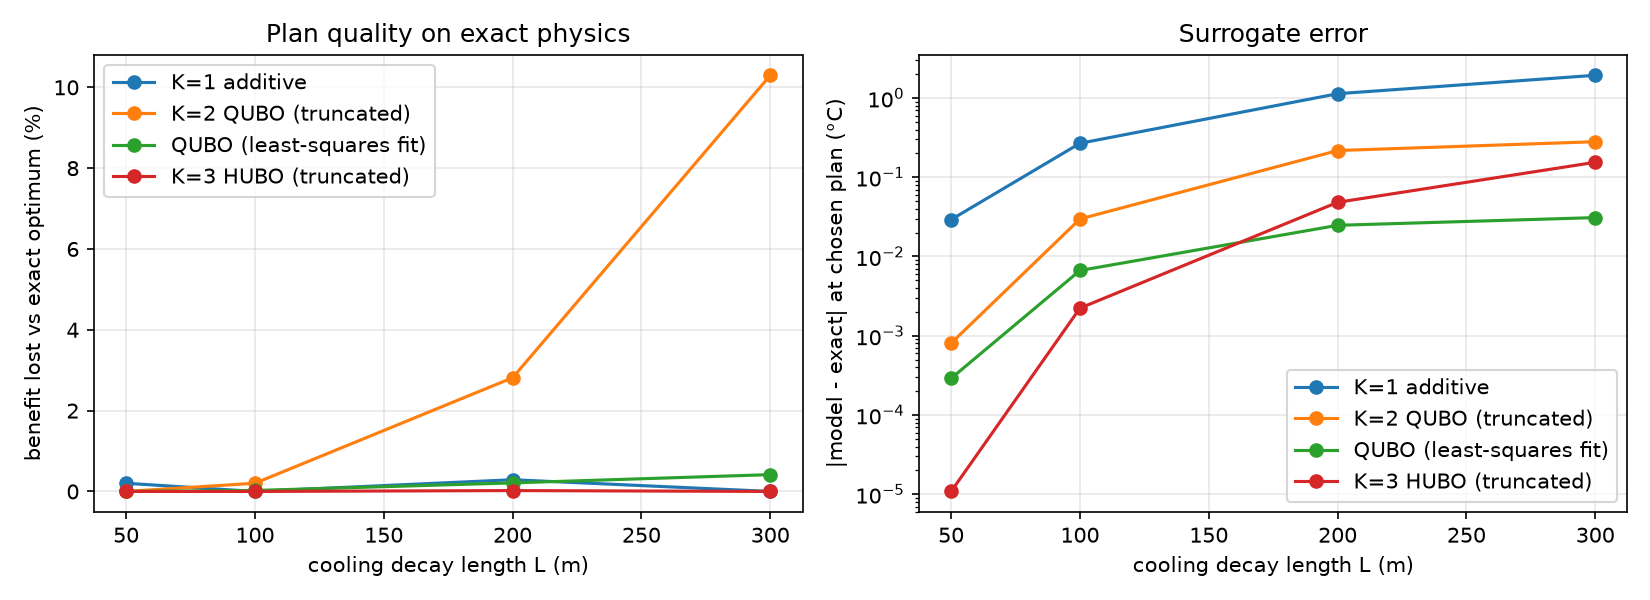
\includegraphics[width=\columnwidth]{e2_fidelity.png}
\caption{E2 surrogate fidelity versus decay length (\code{results/E2\_fidelity/fidelity.png}).}\label{fig:e2}
\end{figure}

\subsection{Classical baselines on penalty models (E3, E7, E9, E10)}
Table~\ref{tab:e3} gives the median raw success probability on the safe-penalty \QUBO{}s. Tabu solves
single-intervention instances up to 27 variables on every read (0.66 at 46), whereas no sampler
reaches the optimum on raw reads of the mix + equity family (42--89 variables). SQA beats SA at
equal sweeps, but SA given as many flip attempts ("SA-matched") is comparable on parks, and SQA's
$+0.02$--$0.03$ benefit on mix + equity costs about 2.4$\times$ the wall time (Fig.~\ref{fig:e3}). The greedy planner
is optimal on 8 of 15 park instances and infeasible on 5 of 9 mix instances. On the E7 showcase
($14\times14$, 81 decision variables, Fig.~\ref{fig:e7}) MILP certifies in 10.8\,s and the greedy
planner returns the same plan, lowering the exposure temperature from 32.311 to 31.141\,\degC{}.

Weak penalties plus repair are the best penalty-based recipe (E9, Table~\ref{tab:e9}): at
$\alpha=0.01$, SA-matched reaches post-processed $\Popt=0.80$ and SQA 0.77, against at most 0.18 at
safe $\Lam$; FeasibleSA reaches 0.46 per read without any penalty, and MILP certifies in 3.8\,s on
average. Slack-free penalties (E10, quick run, Table~\ref{tab:e10}) cut the dynamic range from 163 to
16.5 at $0.1\,\Lsafe$ with an optimal ground state on these two instances, but are not certified in
general.

\begin{table}[!t]
\centering\caption{E3: median raw $\Popt$ per read on safe-penalty \QUBO{}s.}\label{tab:e3}
\resizebox{\columnwidth}{!}{% generated by latex/tools/make_tables.py from results/ -- do not edit
\begin{tabular}{lrrrrrrr}
\toprule
family / vars & Greedy & SA & SA-matched & SQA & SQA-fixedT & Tabu & QAOA(p=4) \\
\midrule
park / 13 & 0.20 & 0.48 & 1.00 & 1.00 & 1.00 & 1.00 & 0.01 \\
park / 17 & 0.06 & 0.03 & 0.48 & 0.56 & 0.84 & 1.00 & -- \\
park / 27 & 0.00 & 0.00 & 0.00 & 0.00 & 0.00 & 1.00 & -- \\
park / 32 & 0.00 & 0.00 & 0.00 & 0.00 & 0.00 & 0.94 & -- \\
park / 46 & 0.00 & 0.00 & 0.00 & 0.00 & 0.00 & 0.66 & -- \\
mix+equity / 42 & 0.00 & 0.00 & 0.00 & 0.00 & 0.00 & 0.00 & -- \\
mix+equity / 56 & 0.00 & 0.00 & 0.00 & 0.00 & 0.00 & 0.00 & -- \\
mix+equity / 89 & 0.00 & 0.00 & 0.00 & 0.00 & 0.00 & 0.00 & -- \\
\bottomrule
\end{tabular}
}
\end{table}

\begin{figure}[!t]
\centering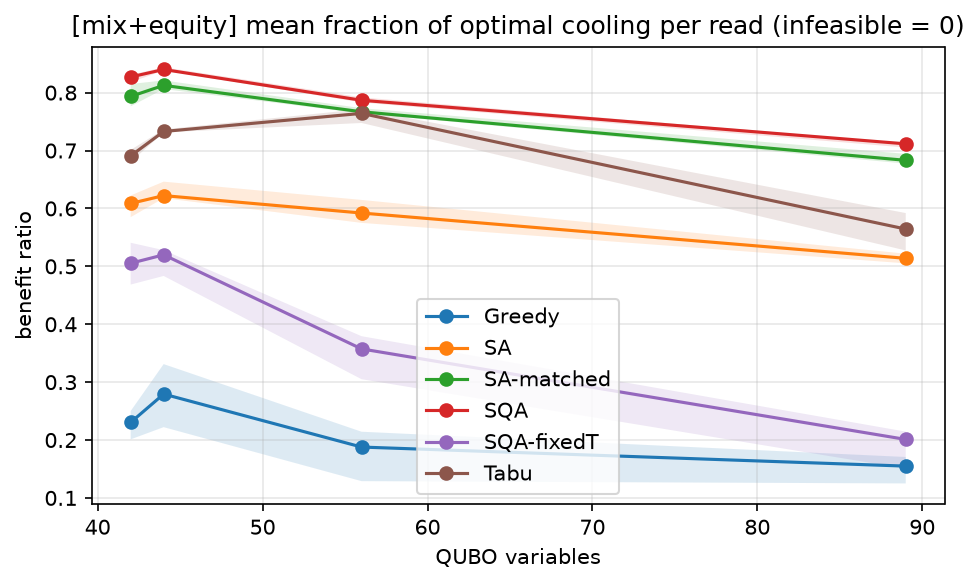
\includegraphics[width=\columnwidth]{e3_benefit_mix.png}
\caption{E3: mean benefit ratio per read versus size on the mix + equity family (\code{results/E3\_scaling/benefit\_vs\_n\_mix\_equity.png}).}\label{fig:e3}
\end{figure}

\begin{table}[!t]
\centering\caption{E9: weak penalty ($\alpha\Lsafe$) plus repair, mix + equity, 9 instances.}\label{tab:e9}
\resizebox{\columnwidth}{!}{% generated by latex/tools/make_tables.py from results/ -- do not edit
\begin{tabular}{llrrrr}
\toprule
solver & $\alpha$ & P(feas) & P(opt) raw & P(opt) pp & benefit pp \\
\midrule
FeasibleSA & -- & 1.000 & 0.460 & -- & -- \\
Greedy planner & -- & 0.444 & 0.444 & -- & -- \\
MILP (HiGHS) & -- & 1.000 & 1.000 & -- & -- \\
SA & 0.01 & 0.608 & 0.017 & 0.503 & 0.941 \\
SA & 1 & 0.979 & 0.000 & 0.031 & 0.813 \\
SA-matched & 0.01 & 0.715 & 0.168 & 0.804 & 0.976 \\
SA-matched & 1 & 1.000 & 0.003 & 0.184 & 0.896 \\
SQA & 0.01 & 0.833 & 0.156 & 0.767 & 0.979 \\
SQA & 1 & 1.000 & 0.003 & 0.108 & 0.880 \\
Tabu & 0.01 & 0.792 & 0.078 & 0.321 & 0.903 \\
Tabu & 1 & 0.983 & 0.000 & 0.009 & 0.748 \\
\bottomrule
\end{tabular}
}
\end{table}

\begin{table}[!t]
\centering\caption{E10: penalty forms (quick run, 2 instances).}\label{tab:e10}
\resizebox{\columnwidth}{!}{% generated by latex/tools/make_tables.py from results/ -- do not edit
\begin{tabular}{llrrrrr}
\toprule
form & weight & vars & dyn.\ range & ground feas. & ground opt. & P(opt) pp \\
\midrule
quadratic slack (exact) & Λ\_safe & 13 & 163.0 & 1.000 & 1.000 & 0.719 \\
unbalanced & 0.1·Λ\_safe & 10 & 16.5 & 1.000 & 1.000 & 0.859 \\
unbalanced & 0.3·Λ\_safe & 10 & 49.0 & 1.000 & 1.000 & 0.766 \\
unbalanced & 1.0·Λ\_safe & 10 & 163.0 & 1.000 & 1.000 & 0.812 \\
linear & 0.5·μ & 10 & 0.6 & 0.000 & 0.000 & 1.000 \\
linear & 1.0·μ & 10 & 0.4 & 0.500 & 0.500 & 0.500 \\
linear & 2.0·μ & 10 & 1.0 & 1.000 & 0.000 & 1.000 \\
\bottomrule
\end{tabular}
}
\end{table}

\begin{figure*}[!t]
\centering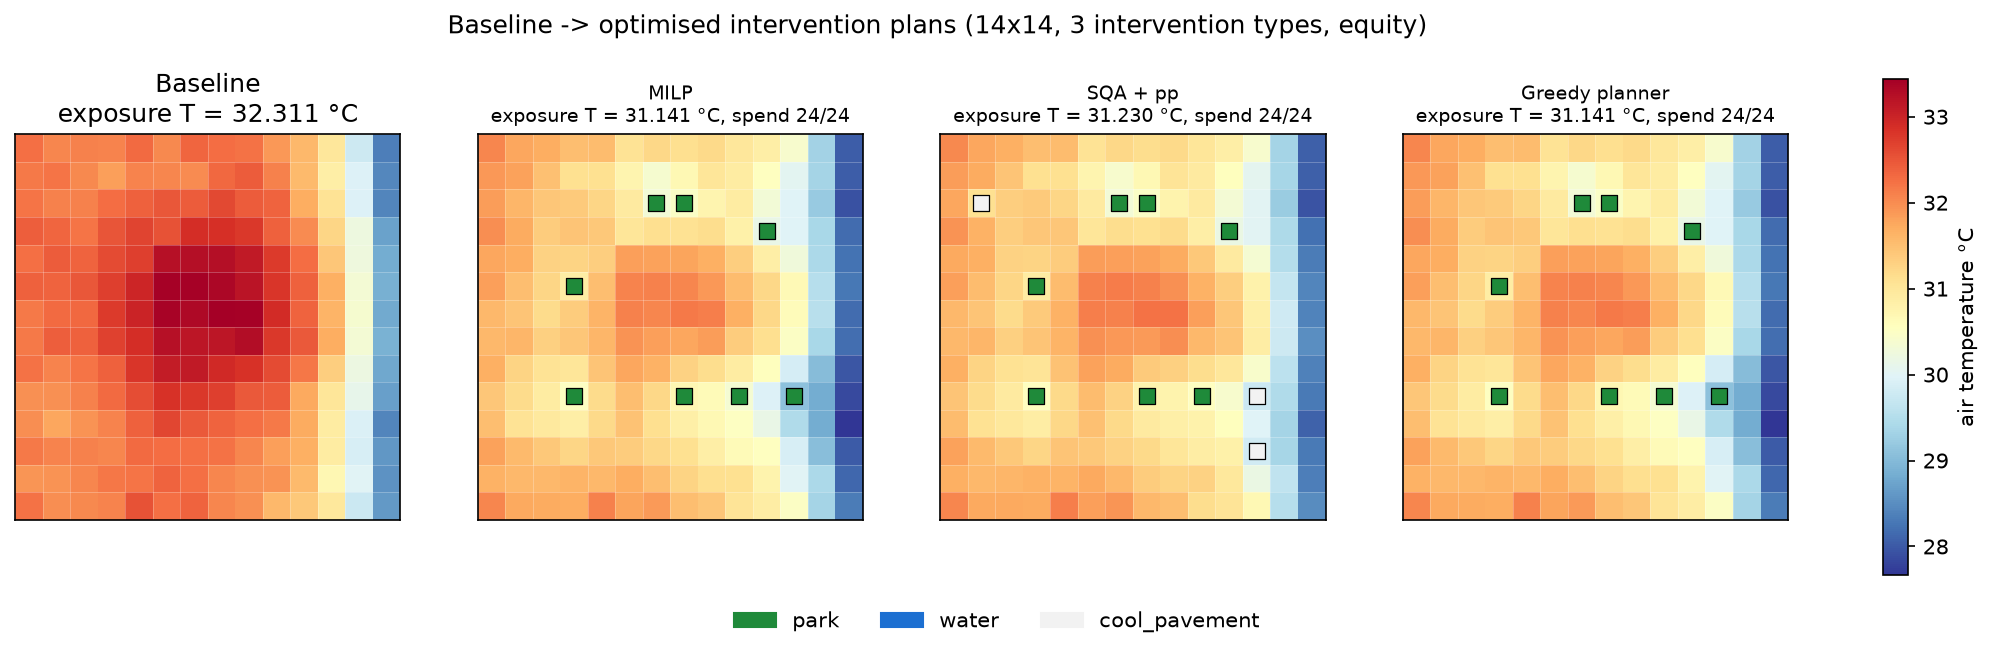
\includegraphics[width=\textwidth]{e7_transition.png}
\caption{E7 showcase: baseline to optimised plans on a $14\times14$ city with three intervention types and equity (\code{results/E7\_showcase/transition.png}).}\label{fig:e7}
\end{figure*}

\subsection{The penalty sets the analog gap (E4, E6)}
On a 14-qubit instance the minimum gap of $H(s)=-(1-s)\sum X+sH_P$ sits at $s=1$ and scales as
$1/\Lam$: $\gap=7.1\times10^{-5}$ at $0.1\,\Lsafe$ and $7.1\times10^{-7}$ at $10\,\Lsafe$
(Table~\ref{tab:e6}, Fig.~\ref{fig:e6}). The adiabatic scale $1/\Delta^2$~\cite{albash2018} therefore grows from
$2.0\times10^{8}$ to $2.0\times10^{12}$. X-mixer QAOA at $p=6$ places 0.17--0.19\% of its
probability on the optimum while reporting an approximation ratio of about 0.998, a number that
mostly measures ``feasible and low penalty''. Weak penalties help samplers but give up
certification: $0.01\,\Lsafe$ plus repair lifts post-processed $\Popt$ from at most 0.03 to 0.42--0.47
on a mix + equity instance (E4, Fig.~\ref{fig:e4}).

\begin{figure}[!t]
\centering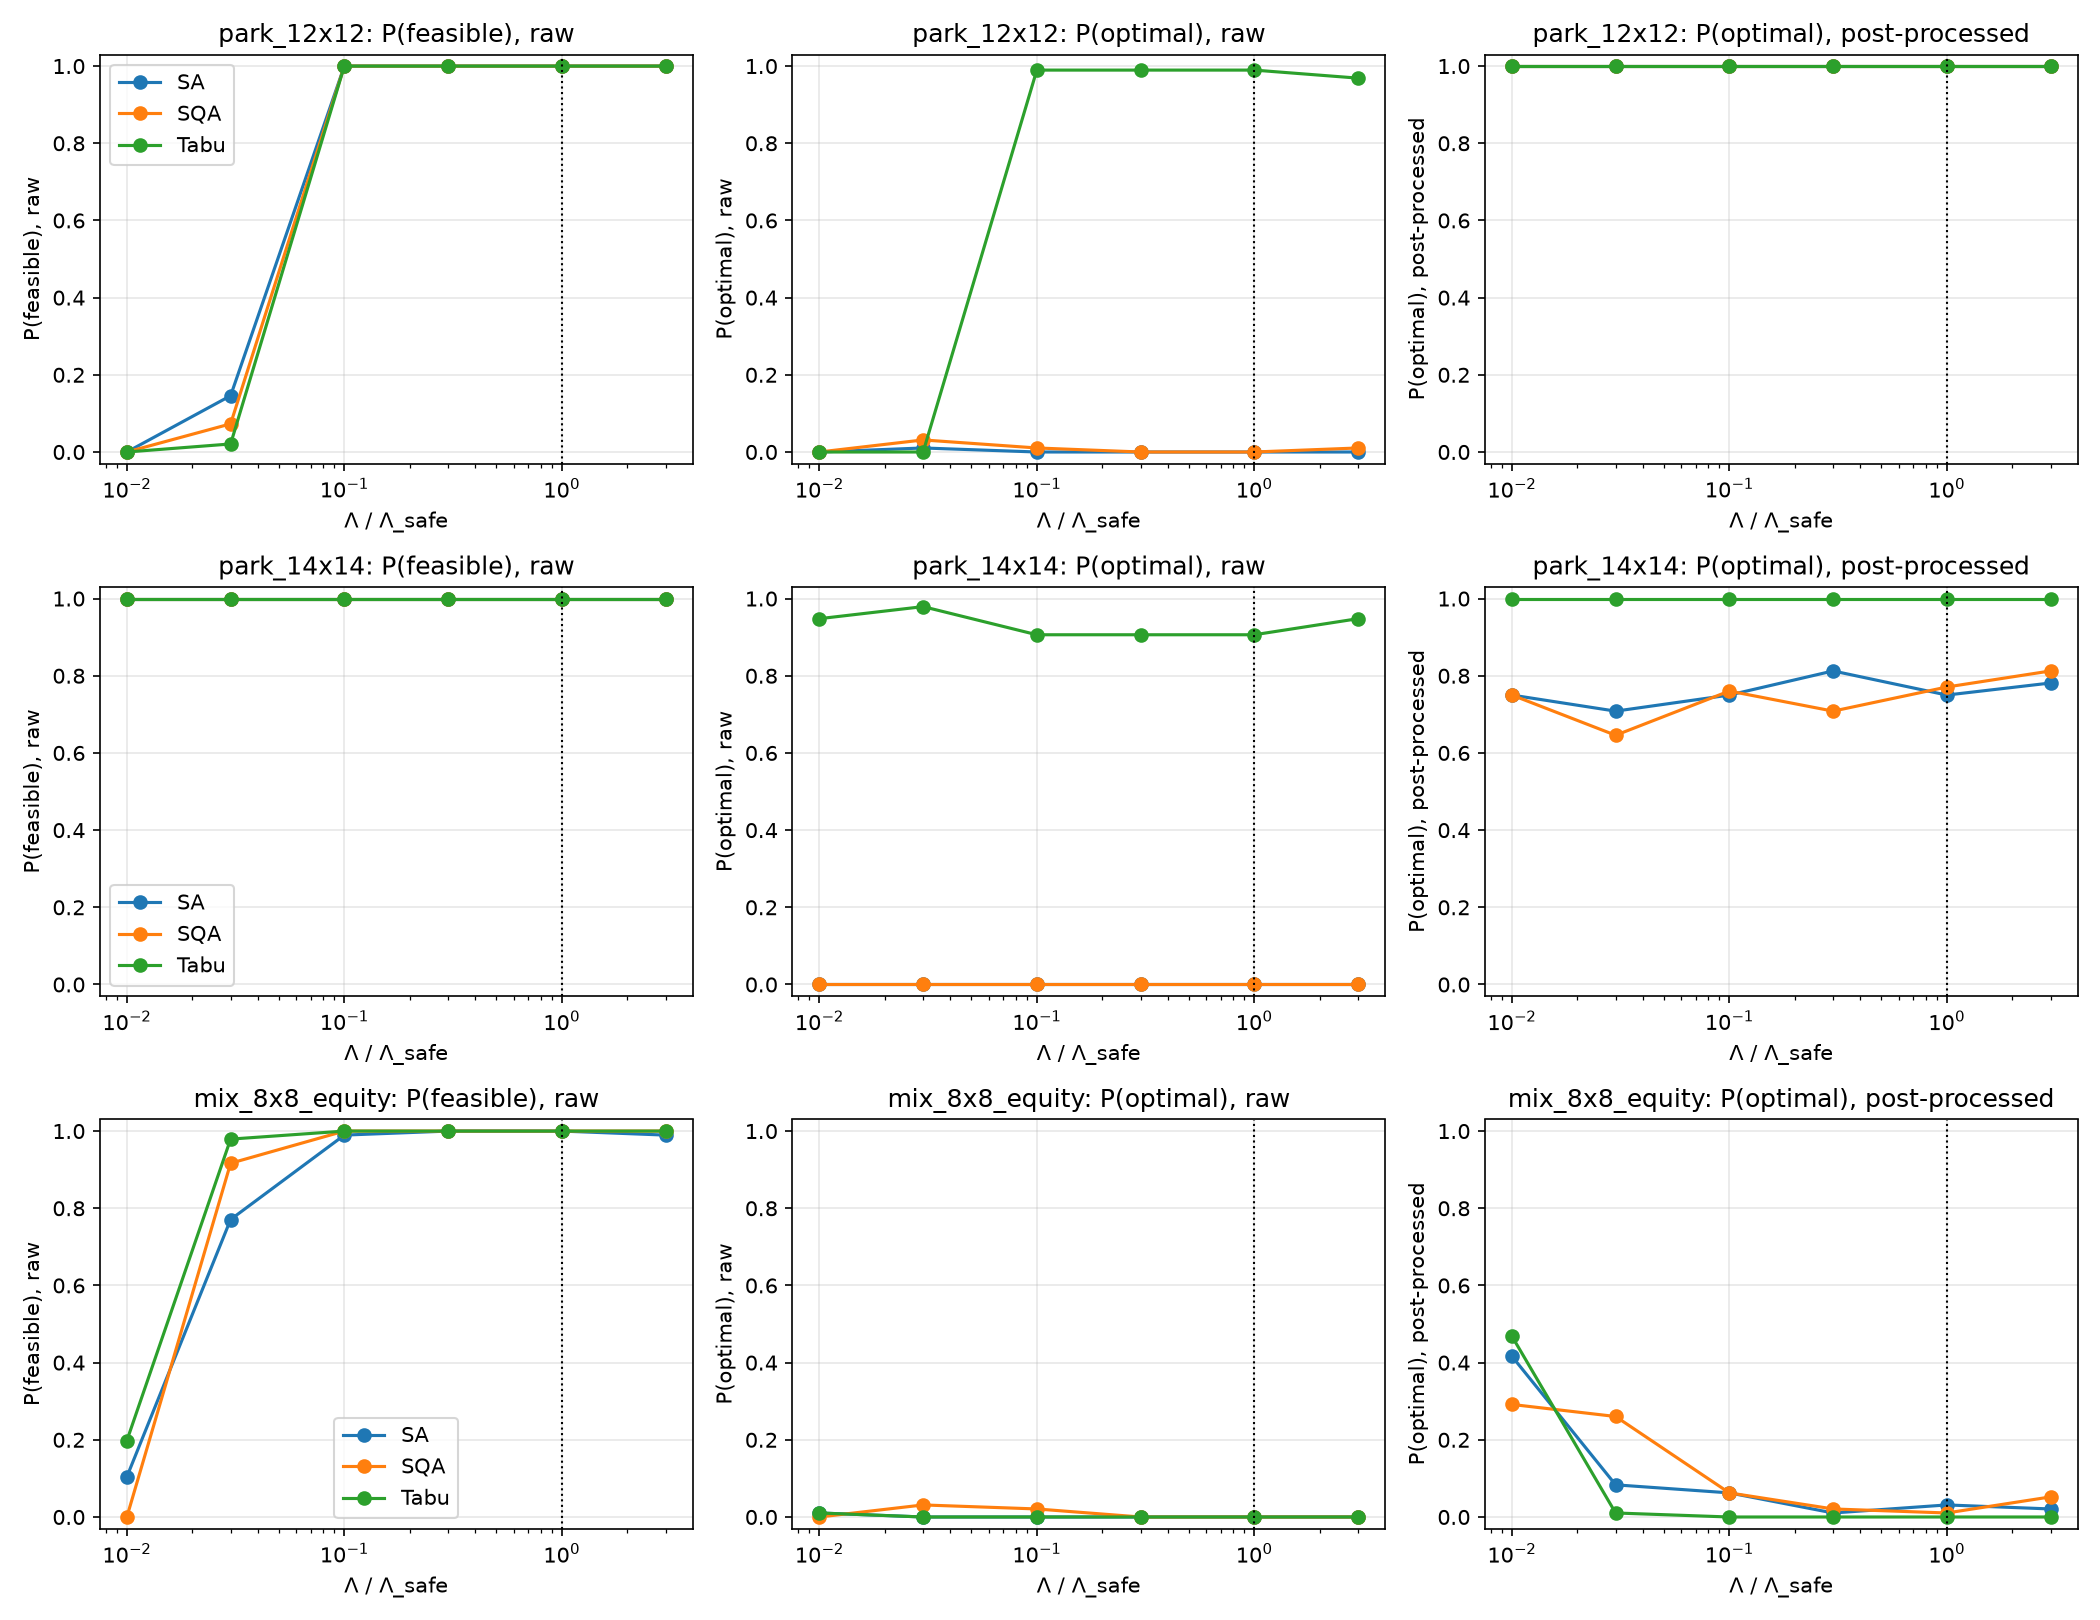
\includegraphics[width=\columnwidth]{e4_penalty_sweep.png}
\caption{E4: raw and post-processed feasibility and success versus $\Lam/\Lsafe$ (\code{results/E4\_penalty/penalty\_sweep.png}).}\label{fig:e4}
\end{figure}

\begin{table}[!t]
\centering\caption{E6: 14-qubit spectra and QAOA versus penalty weight.}\label{tab:e6}
\resizebox{\columnwidth}{!}{% typed from docs/RESULTS.md (E6; source results/E6_quantum/quantum_small.csv)
\begin{tabular}{lcccc}
\toprule
$\Lam/\Lsafe$ & ground = opt. & $\gap$ & $1/\Delta^2$ & QAOA $\Popt$, $p{=}6$ \\
\midrule
0.1 & yes & $7.1\times10^{-5}$ & $2.0\times10^{8}$ & 0.0019 \\
0.3 & yes & $2.4\times10^{-5}$ & $1.8\times10^{9}$ & 0.0018 \\
1 & yes & $7.1\times10^{-6}$ & $2.0\times10^{10}$ & 0.0017 \\
3 & yes & $2.4\times10^{-6}$ & $1.8\times10^{11}$ & 0.0017 \\
10 & yes & $7.1\times10^{-7}$ & $2.0\times10^{12}$ & 0.0017 \\
\bottomrule
\end{tabular}
}
\end{table}

\begin{figure}[!t]
\centering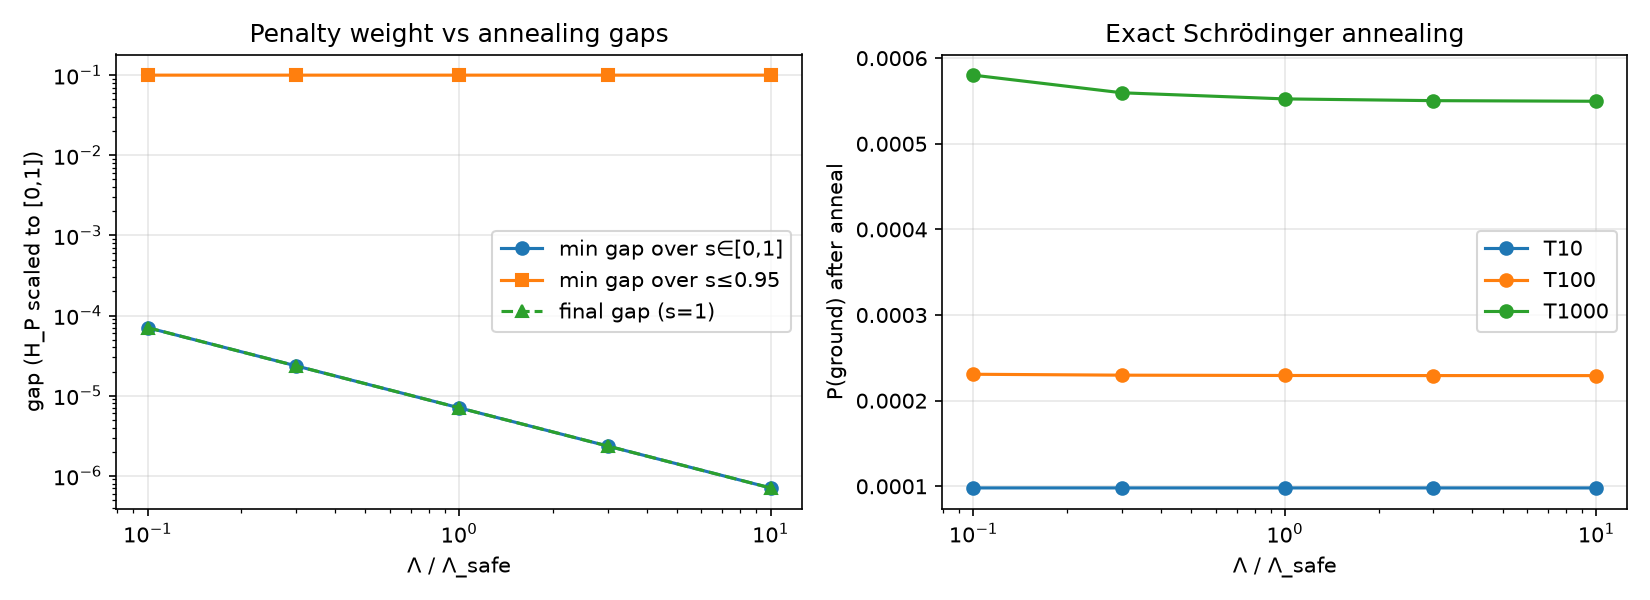
\includegraphics[width=\columnwidth]{e6_gap_vs_penalty.png}
\caption{E6: final gap and adiabatic scale versus penalty weight (14 qubits).}\label{fig:e6}
\end{figure}

\subsection{Constraint-preserving QAOA (E8, E8b)}
Dicke/XY mixers keep the state feasible and raise $\Popt$ 10--70$\times$ over X-mixer penalty QAOA
at equal depth (E8). They do not reach the classical bar. Table~\ref{tab:e8b} and
Fig.~\ref{fig:e8b} show the depth curve on three ``exactly 3 parks'' cities ($|\Fset|=120$):
Dicke-XY complete rises from 0.134 at $p=1$ to 0.427 at $p=6$ (maximum 0.65), while FeasibleSA
returns the optimum in every run in 0.21\,s. Mixer connectivity matters more than depth: ring-XY at
$p=6$ (0.111) is below complete-XY at $p=1$. On mix + equity, XY-QAOA at $p=2$ reaches $\Popt=0.003$
(benefit 0.61) against FeasibleSA's 0.39 (benefit 0.92).

\begin{table}[!t]
\centering\caption{E8b: exact $\Popt$ vs QAOA depth, mean [min--max] over 3 cities.}\label{tab:e8b}
\resizebox{\columnwidth}{!}{% generated by latex/tools/make_tables.py from results/ -- do not edit
\begin{tabular}{lrrrrr}
\toprule
method & $p{=}1$ & $p{=}2$ & $p{=}3$ & $p{=}4$ & $p{=}6$ \\
\midrule
Dicke-XY complete & 0.134 & 0.242 [0.08--0.37] & 0.309 & 0.376 & 0.427 [0.17--0.65] \\
Dicke-XY ring & 0.034 & 0.067 [0.02--0.14] & 0.057 & 0.066 & 0.111 [0.02--0.26] \\
X-mixer penalty QAOA & 0.004 & 0.005 & 0.006 & 0.008 & 0.009 \\
\bottomrule
\end{tabular}
}\\[4pt]
\footnotesize% generated by latex/tools/make_tables.py from results/ -- do not edit
\begin{tabular}{lrrr}
\toprule
method & \Popt & benefit & wall (s) \\
\midrule
MILP (HiGHS) & 1.000 & 1.000 & 0.317 \\
Greedy planner & 0.667 & 1.000 & $8.54\times10^{-4}$ \\
uniform on F & 0.008 & 0.849 & 0.000 \\
FeasibleSA & 1.000 & 1.000 & 0.206 \\
\bottomrule
\end{tabular}

\end{table}

\begin{figure}[!t]
\centering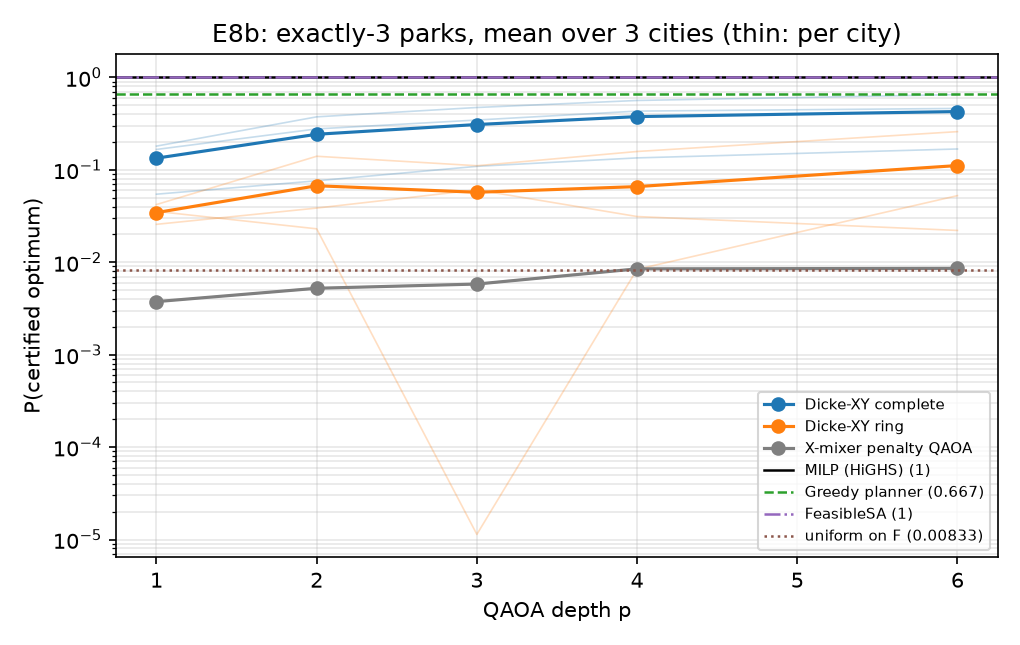
\includegraphics[width=\columnwidth]{p_opt_vs_p.png}
\caption{E8b: $\Popt$ versus depth $p$ for Dicke-XY complete and ring mixers and the X-mixer penalty control.}\label{fig:e8b}
\end{figure}

\subsection{Feasible-space PIMC and its ablation (E12, E12b)}
Family H has nine mix + equity instances on $8\times8$ to $12\times12$ grids with a budget equal to
the grid side. Under a matched wall-clock $\Tstar$ per run (1.4--20\,s), FeasibleSQA reaches a mean
$\btrue$ of 0.981 and passes the pre-committed rule (Table~\ref{tab:e12}). So do FeasibleSA (0.973)
and Tabu-on-F (0.976); the greedy planner is infeasible on 6 of 9 instances; ConstrainedQAOA (0.658
at $p=2$, 0.665 at $p=4$) fits only the $8\times8$ cities, and MILP reaches 1.000 in 0.81\,s.

The ablation explains the ordering. HiGHS never set $\Tstar$, so the clock was not padded; instead,
FeasibleSQA made 3.6$\times$ as many proposals in the same time (4.66\,M against 1.30\,M per run),
because moves that would leave $\Fset$ are rejected before $f$ is evaluated. At an equal budget of
4.53\,M proposals per run, FeasibleSA scores 0.988 and FeasibleSQA 0.983 (ahead on 1 instance, tied
on 6, behind on 2; Table~\ref{tab:e12b}). FeasibleSQA is within 5\% of FeasibleSA; it is not ahead. FeasibleSQA needs less wall-clock per
proposal (7.1\,s against 25.0\,s for the same count), an implementation property of early
rejection, not a quantum effect. Tabu-on-F does not improve with more work (0.977 on both clocks),
and QAOA-seeded FeasibleSA still loses the $|\Fset|=2484$ city on the tight clock because the
subspace simulation alone exceeds it. Fig.~\ref{fig:e12} places every E12 method on the
benefit--time plane.

\begin{figure*}[!t]
\centering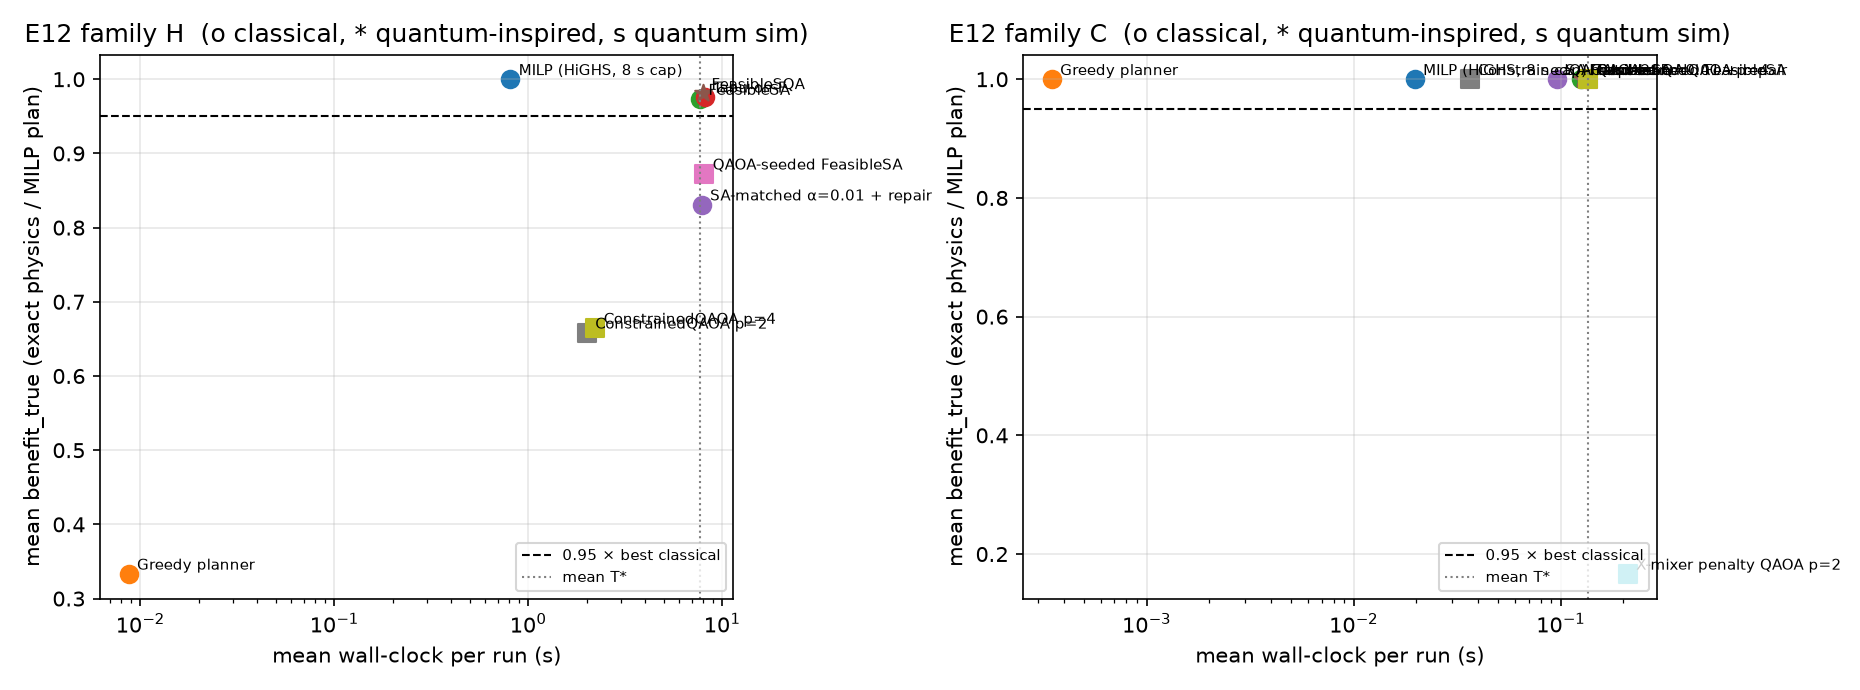
\includegraphics[width=0.9\textwidth]{e12_benefit_vs_time.png}
\caption{E12: mean $\btrue$ versus mean wall-clock per run for family H (left) and the park control C (right); the dashed line is 0.95 of the best classical mean (\code{results/E12\_comparable/benefit\_vs\_time.png}).}\label{fig:e12}
\end{figure*}

\begin{table*}[!t]
\centering
\begin{minipage}[!t]{0.47\textwidth}\centering
\caption{E12 family H at matched wall-clock $\Tstar$.}\label{tab:e12}
\resizebox{\linewidth}{!}{% generated by latex/tools/make_tables.py from results/ -- do not edit
\begin{tabular}{lrrrrrc}
\toprule
method (family H) & P(feas) & \Popt & benefit & min & wall (s) & comp. \\
\midrule
MILP (HiGHS, 8 s cap) & 1.000 & 1.000 & 1.000 & 1.000 & 0.809 & yes \\
Greedy planner & 0.333 & 0.333 & 0.333 & 0.000 & 0.009 & no \\
FeasibleSA & 1.000 & 0.778 & 0.973 & 0.813 & 7.693 & yes \\
Tabu-on-F & 1.000 & 0.778 & 0.976 & 0.708 & 8.120 & yes \\
SA-matched α=0.01 + repair & 0.833 & 0.722 & 0.831 & 0.000 & 7.847 & no \\
FeasibleSQA & 1.000 & 0.722 & 0.981 & 0.854 & 7.975 & yes \\
QAOA-seeded FeasibleSA & 1.000 & 0.833 & 0.873 & 0.000 & 8.095 & no \\
ConstrainedQAOA p=2 & 1.000 & 0.500 & 0.658 & 0.000 & 2.008 & no \\
ConstrainedQAOA p=4 & 1.000 & 0.167 & 0.665 & 0.000 & 2.221 & no \\
\bottomrule
\end{tabular}
}
\end{minipage}\hfill
\begin{minipage}[!t]{0.51\textwidth}\centering
\caption{E12b family H at equal proposals $\Wstar$.}\label{tab:e12b}
\resizebox{\linewidth}{!}{% generated by latex/tools/make_tables.py from results/ -- do not edit
\begin{tabular}{llrrrrrc}
\toprule
method & clock & \Popt & benefit & min & wall (s) & prop.\ (M) & w/t/l \\
\midrule
MILP (HiGHS, 8 s cap) & none & 1.000 & 1.000 & 1.000 & 0.77 & -- & -- \\
FeasibleSA & equal\_work & 0.889 & 0.988 & 0.854 & 24.99 & 4.53 & -- \\
Tabu-on-F & equal\_work & 0.833 & 0.977 & 0.708 & 11.32 & 4.65 & 1/6/2 \\
FeasibleSQA & equal\_work & 0.778 & 0.983 & 0.813 & 7.09 & 4.53 & 1/6/2 \\
QAOA-seeded FeasibleSA & equal\_work & 1.000 & 1.000 & 1.000 & 2.28 & 2.20 & 0/3/0 \\
\bottomrule
\end{tabular}
}
\end{minipage}
\end{table*}

\subsection{An LST-shaped tile (E13)}
A $16\times16$ tile with a compact hot core, population on the core and only 2 candidate lots left
in the core ($n=108$, $|\Fset|>4000$) did not create a classical gap (Table~\ref{tab:e13}). HiGHS
certifies it in 1.67\,s; greedy fails on equity; the weak-penalty hybrid finds the optimum on both
seeds. FeasibleSQA (0.9998) above FeasibleSA (0.9569) on two tight-clock seeds is not evidence of an
advantage, for the reason E12b gives. Fig.~\ref{fig:e13} shows the tile and the returned plans;
Tabu-on-F falls to 0.37 on one seed.

\begin{figure*}[!t]
\centering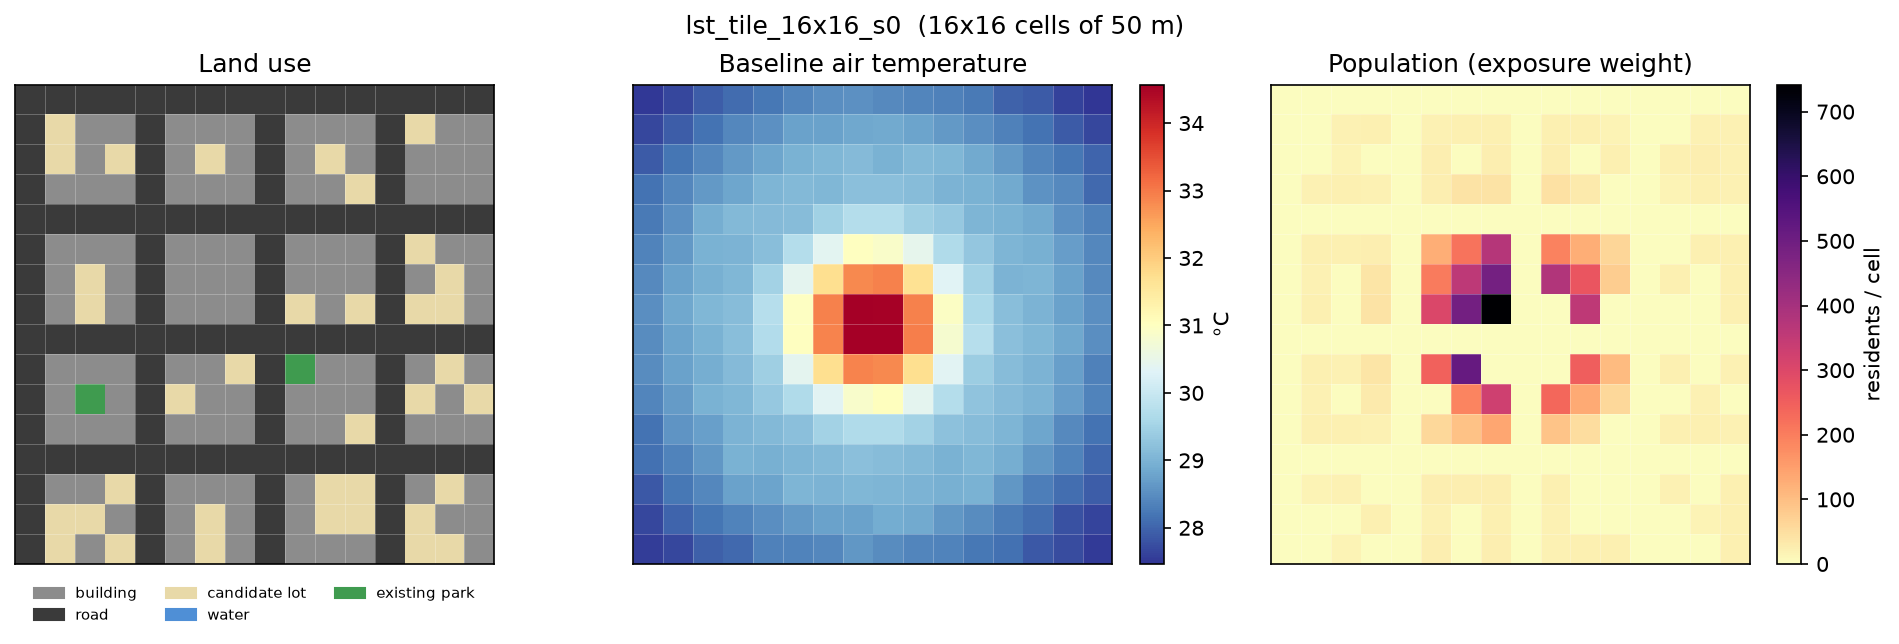
\includegraphics[width=0.8\textwidth]{e13_city.png}\\[2pt]
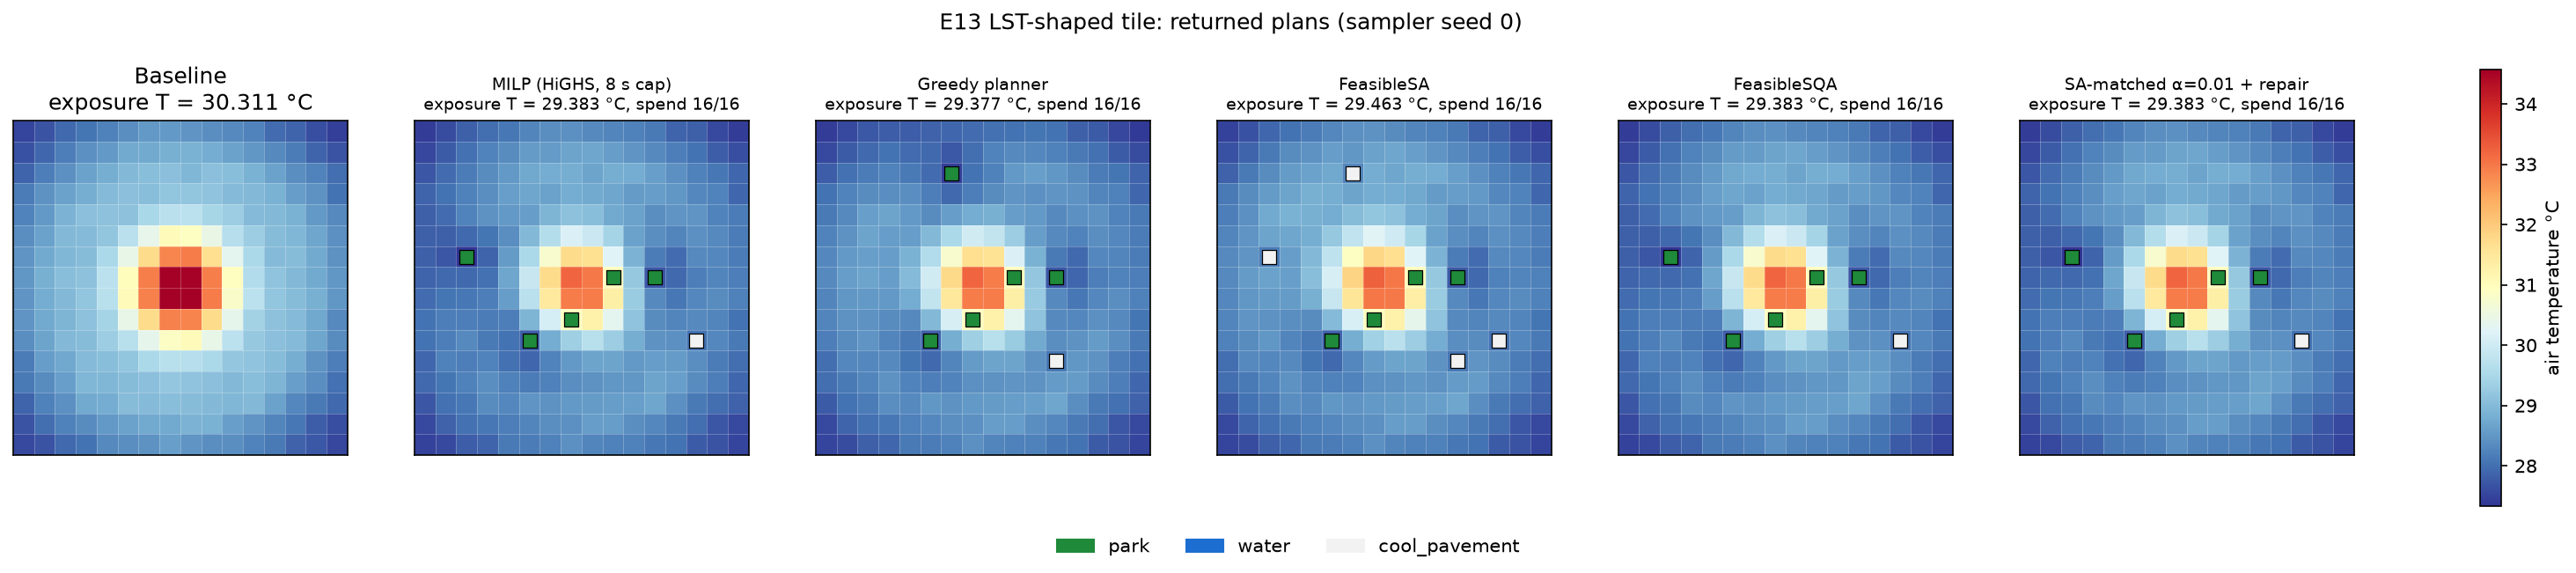
\includegraphics[width=\textwidth]{e13_plans.png}
\caption{E13: the LST-shaped tile (land use, baseline temperature, population) and the plans returned by MILP, greedy, FeasibleSA, FeasibleSQA and the weak-penalty hybrid (sampler seed 0).}\label{fig:e13}
\end{figure*}

\begin{table}[!t]
\centering\caption{E13 LST-shaped tile, tight clock 68.59\,s, two seeds.}\label{tab:e13}
\footnotesize% generated by latex/tools/make_tables.py from results/ -- do not edit
\begin{tabular}{lrrrr}
\toprule
method & P(feas) & \Popt & benefit & wall (s) \\
\midrule
MILP (HiGHS, 8 s cap) & 1.0 & 1.0 & 1.0000 & 1.67 \\
Greedy planner & 0.0 & 0.0 & 0.0000 & 0.06 \\
FeasibleSA & 1.0 & 0.5 & 0.9569 & 66.56 \\
Tabu-on-F & 1.0 & 0.0 & 0.6412 & 67.35 \\
FeasibleSQA & 1.0 & 0.5 & 0.9998 & 63.72 \\
SA-matched α=0.01 + repair & 1.0 & 1.0 & 1.0000 & 64.68 \\
\bottomrule
\end{tabular}

\end{table}

\begin{figure*}[!t]
\centering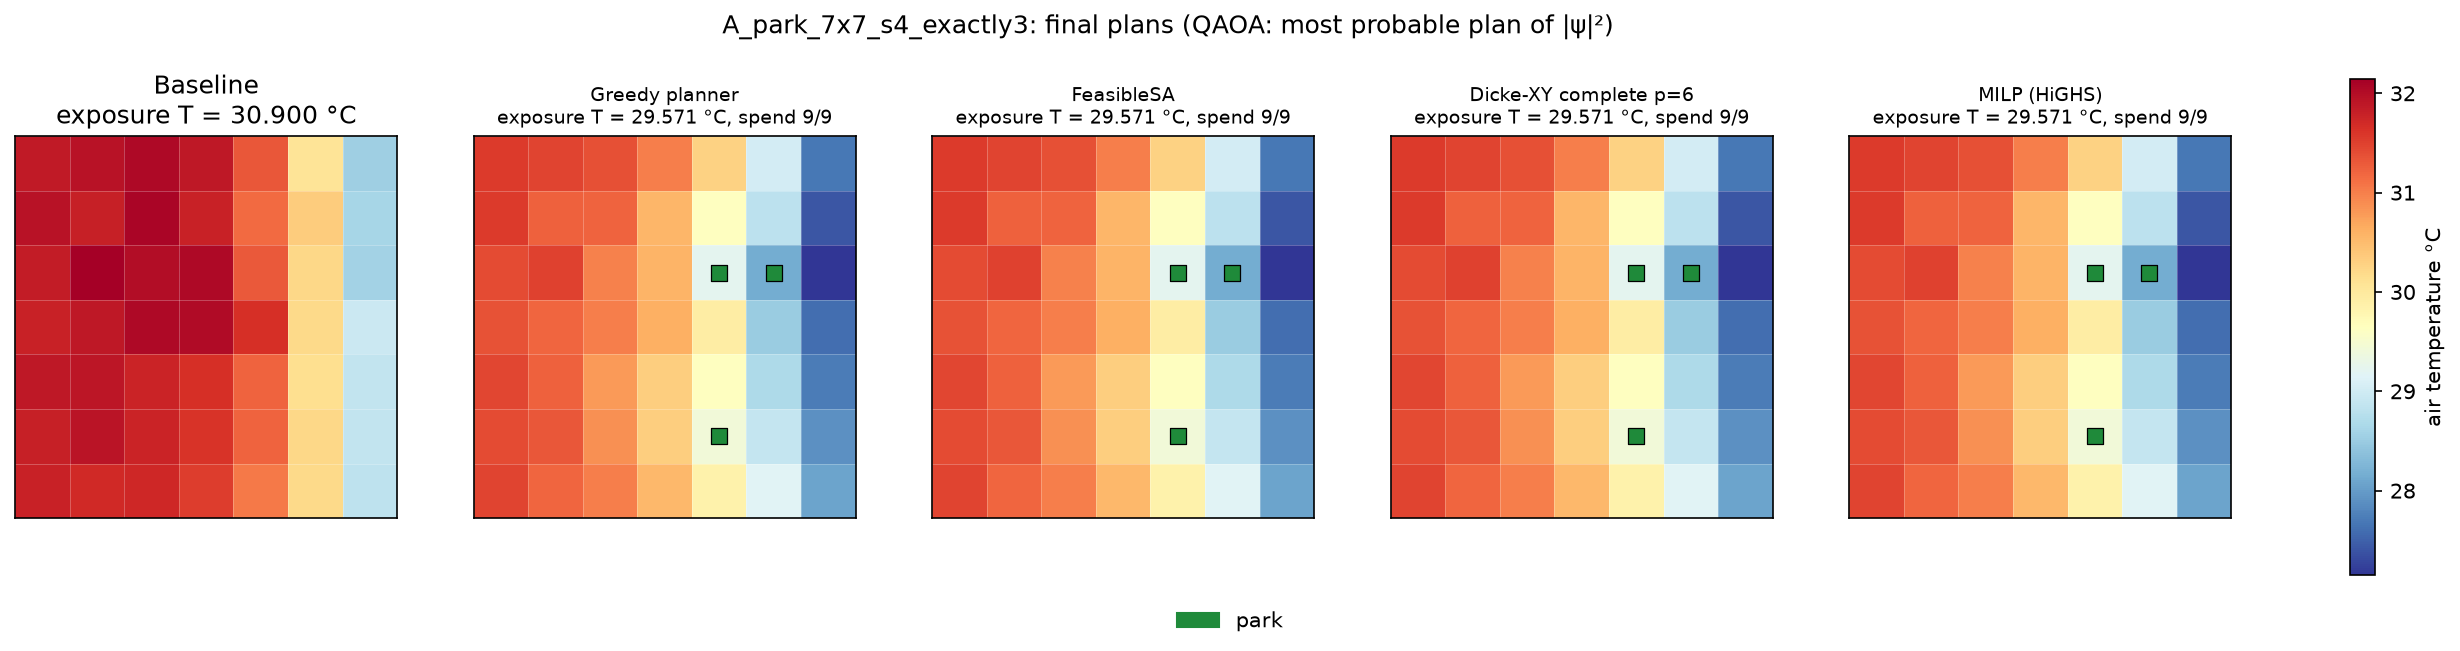
\includegraphics[width=\textwidth]{compare_final.png}
\caption{Final plans on the E8b ``exactly 3 parks'' city: greedy, FeasibleSA, Dicke-XY $p=6$ (most probable plan) and MILP, on one locked temperature scale. Animated versions are supplementary: \code{results/ANIM/compare\_temp\_A\_park\_7x7\_s4\_exactly3.gif} and \code{results/ANIM/compare\_temp\_B\_mix\_10x10\_s0.gif}.}\label{fig:anim}
\end{figure*}

\begin{figure*}[!t]
\centering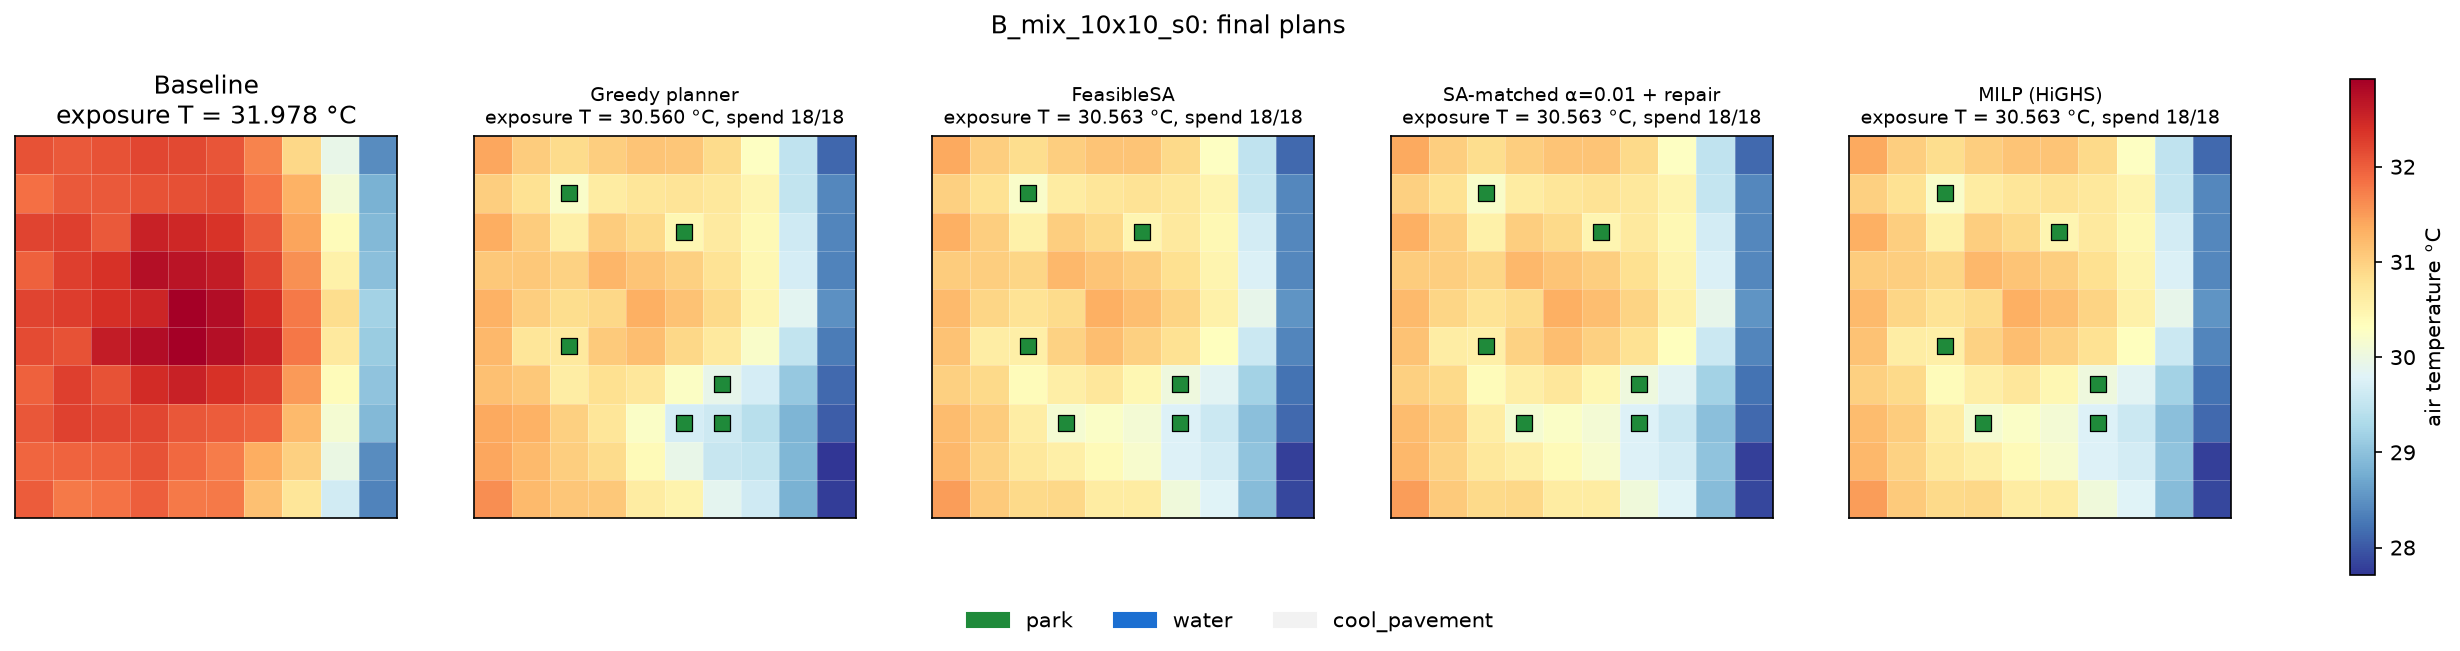
\includegraphics[width=\textwidth]{compare_final_B.png}
\caption{Final plans on the E9 $10\times10$ mix + equity city: greedy (infeasible on equity), FeasibleSA, the weak-penalty hybrid (in place of QAOA, since $|\Fset|>4000$) and MILP.}\label{fig:animB}
\end{figure*}

%======================================================================
\section{Discussion}\label{sec:discussion}
\textbf{Criterion not met.} Gate-model QAOA misses the bar with penalties (it learns the constraint,
not the objective) and with constraint-preserving mixers (it stays well below FeasibleSA and MILP at
every simulated depth). Feasible-space PIMC only ties feasible-space SA.

\textbf{Encodings decide.} Every improvement to a quantum or quantum-inspired method in this study
was an encoding change: certified but gentler penalties, native higher-order terms, and moves or
mixers that respect the constraints. Each helped the classical methods at least as much.

\textbf{Hold-ups, in order of impact.} (i) Slack penalties compress the objective, so the
analog gap scales as $1/\Lam$ (E6, E11). (ii) Quadratisation multiplies variables 6.4$\times$ and
blocks single-flip dynamics (E5). (iii) At equal work, PIMC advantages over SA vanish (E3, E9,
E12b). (iv) The objective is submodular, so greedy is strong wherever equity does not bind.
(v) Constraint-preserving mixers fix feasibility but not optimality at simulable depths (E8b).
(vi) QAOA approximation ratios near 1 are cosmetic on penalty-dominated scales (E6). (vii) No
constrained model was run on a QPU or hybrid solver.

\textbf{What hardware could test.} A fair test would send the constrained model natively, as a CQM
to a hybrid solver, on the E8b ``exactly 3'' city and a park-only control city. A safe-$\Lam$ slack
\QUBO{} should not be sent to a QPU, because its gap is set by $\Lam$. No D-Wave result exists in
this work; the repository hook is inactive without an API token.

%======================================================================
\section{Limitations}\label{sec:limitations}
Cities and the E13 tile are synthetic, with illustrative intervention parameters; the saturation law
is a surrogate for CFD, and MILP certifies the $K{=}2$ surrogate. SQA and FeasibleSQA are PIMC, not
hardware quantum annealing~\cite{heim2015}. ConstrainedQAOA is a subspace simulation on
$\mathrm{span}(\Fset)$, not a compiled circuit. E12/E12b use three instances and two seeds per cell,
and E10/E11 are quick runs on two instances.

\section*{Reproducibility}
Every table is generated from the committed CSVs by \code{latex/tools/make\_tables.py};
experiments rerun with \code{python scripts/run\_experiments.py --only E$k$}, and the legacy audit
with \code{python scripts/audit\_legacy.py}. Animated comparisons are in \code{results/ANIM/}.

\section*{Acknowledgements}
{\sloppy
The experiments, the toolkit and this manuscript were produced in the \repo{} repository
(branch \code{claude/clever-gates-ezote4}, commit \sha). No external data, cloud solver or
quantum hardware was used.\par}


\clearpage
\bibliographystyle{IEEEtran}
\bibliography{../bib/refs}
\end{document}
